\documentclass[tikz]{standalone}
\begin{document}
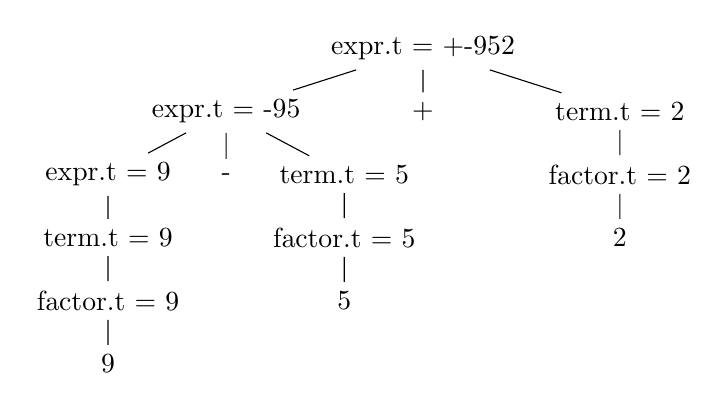
\begin{tikzpicture}[level 1/.style={level distance=8mm, sibling distance=25mm},
                    level 2/.style={level distance=8mm, sibling distance=15mm}]
  \node {expr.t = +-952}
    child { node {{expr.t = -95} }
      child { node {expr.t = 9}
        child { node {term.t = 9}
          child { node {factor.t = 9}
            child { node {9} }
          }
        }
      }
      child { node {-} }
      child { node {term.t = 5}
        child { node {factor.t = 5}
          child { node {5} }
        }
      }
    }
    child { node {+} }
    child { node {term.t = 2}
      child { node {factor.t = 2}
        child { node {2} }
      }
    }
  ;
\end{tikzpicture}
\end{document}
